\fancypagestyle{plain}{\fancyhead{}\renewcommand{\headrulewidth}{0pt}}
\chapter{Implementazione}
In questa sezione verrà illustrato il porting di Edge Engine da Arduino ESP32 a dispositivi di tipo PC. Al fine di mantenere il prodotto finale slegato dalla piattaforma, si è scelto di utilizzare il compilatore \textbf{g++}, disponibile su dispositivi Windows, Linux e MacOS.

In primo luogo verrà discussa l’installazione delle librerie POCO, necessarie per usufruire delle HTTP requests, per poi passare alla modifica del codice preesistente affinché possa essere eseguito sul target desiderato, mantenendo però la compatibilità con dispositivi Arduino. In ultimo, verranno mostrati un possibile esempio di utilizzo e la creazione di una libreria vera e propria, al fine di permettere una diffusione su più larga scala unita ad una facilità d'uso maggiore.
\section{Librerie POCO}
Come anticipato in precedenza, la prima versione di Edge Engine, in quanto prevista per Arduino, è dotata di due classi wrapper, \texttt{Connection} e \texttt{APIRest}, adibite alla gestione di risorse hardware e, pertanto, legate alla piattaforma in uso. Di conseguenza, si è resa necessaria la creazione di altre due classi che permettessero di svolgere le stesse funzioni su dispositivi PC. Dal momento che le due classi necessitano di effettuare HTTP requests o di accedere alla rete Internet e l’obbiettivo del progetto è quello di mantenere il più possibile il codice indipendente dalla piattaforma, si è scelto di fare affidamento sulle librerie POCO \cite{POCO}.
\subsection{Installazione}
Le librerie POCO sono un potente strumento C++ multipiattaforma per la creazione di applicazioni basate su rete e Internet che funzionano su desktop, server, dispositivi mobili, IoT e sistemi integrati.

L’installazione di queste librerie, tuttavia, si è rivelata più complicata del previsto, dal momento che la documentazione riguardante la compilazione delle stesse facendo uso di g++ è quasi del tutto assente.

\subsubsection{VCPKG, CMake, Conan}
In primo luogo, come da istruzioni del sito POCO, si è tentata l’installazione attraverso il package manager VCPKG \cite{VCPKG}: un gestore di pacchetti open source multipiattaforma di Microsoft. Nonostante VCPKG riportasse il supporto alla compilazione di tali librerie tramite g++, il processo si interrompeva intorno al 70\% a causa del seguente errore:

\begin{verbatim}
In file included 
  from C:/mingw/mingw64/x86_64-w64-mingw32/include/mprapi.h:16       
  from C:/mingw/mingw64/x86_64-w64-mingw32/include/iprtrmib.h:12,
  from C:/mingw/mingw64/x86_64-w64-mingw32/include/Iphlpapi.h:15,
  from C:/poco/Foundation/include/Poco/UnWindows.h:33,
  from C:/poco/Foundation/include/Poco/Platform_WIN32.h:22,
  from C:/poco/Foundation/include/Poco/Foundation.h:100,
  from C:/poco/Net/include/Poco/Net/ICMPPacket.h:21,
  from C:\poco\Net\src\ICMPPacket.cpp:15:
C:/poco/Net/include/Poco/Net/ICMPv4PacketImpl.h:72:3: error: 
expected identifier before '(' token
   TIMESTAMP_REQUEST,
   ^~~~~~~~~~~~~~~~~
   
   [...]
   
mingw32-make.exe[2]: *** [Net\CMakeFiles\Net.dir\build.make:679:
Net/CMakeFiles/Net.dir/src/ICMPPacket.cpp.obj] Error 1
mingw32-make.exe[1]: *** [CMakeFiles\Makefile2:530: 
Net/CMakeFiles/Net.dir/all] Error 2
mingw32-make.exe: *** [Makefile:151: all] Error 2
\end{verbatim}

Il secondo tentativo è stato invece effettuato utilizzando CMake \cite{CMake}. CMake è un tool modulare che, con poche e concise istruzioni, è in grado di generare Makefile. Esso dispone di una particolare sintassi comprensiva di moltissime macro il cui utilizzo è possibile mediante un apposito file chiamato  \textbf{CMakeLists.txt}. Per la generazione del Makefile e la successiva compilazione del progetto, è necessario eseguire i seguenti comandi:

\begin{verbatim}
mkdir build
cd build
cmake ..
make
\end{verbatim}

Anche in questo caso però, la compilazione si interrompeva attorno al 70\% restituendo lo stesso errore di VCPKG.

A seguito dei primi due tentativi falliti, si è scelto di provare a installare le librerie POCO tramite Conan: un package manager open source per C e C++ che consente ai team di sviluppo di gestire in modo semplice ed efficiente pacchetti e dipendenze tra piattaforme e sistemi di compilazione \cite{Conan}. Il funzionamento di Conan è analogo a quello di VCPKG, ma i file necessari all'installazione delle librerie sono differenti, pertanto ci si sarebbe potuto aspettare un esito differente da quelli passati. Tuttavia, dopo aver seguito le istruzioni specificate dalla guida all'utilizzo, il risultato ottenuto è stato analogo ai precedenti.
\subsubsection{MSYS2}
In ultimo, nonostante non ci fosse alcuna documentazione a riguardo nemmeno sul sito delle librerie POCO, la mancanza di valide alternative ha portato a sperimentare una via differente, rappresentata dal tool MSYS2 \cite{MSYS2}. MSYS2 è una raccolta di strumenti e librerie che fornisce un ambiente di facile utilizzo per la creazione, l'installazione e l'esecuzione di software nativo Windows. Essa offre build aggiornate per GCC, mingw-w64, CPython, CMake, Meson, OpenSSL, ecc. Per fornire una facile installazione dei pacchetti e un modo per mantenerli aggiornati, è dotata di un package manager chiamato Pacman \cite{Pacman}, il quale offre molte potenti funzionalità tra cui la risoluzione delle dipendenze e semplici aggiornamenti di sistema, nonché la creazione di pacchetti. La distribuzione del software MSYS2 utilizza un porting di Pacman per creare e gestire (installare, rimuovere e aggiornare) i pacchetti binari.

Al fine di installare le librerie POCO tramite MSYS2 è necessario eseguire la seguente istruzione sul prompt dei comandi fornito in dotazione:

\begin{verbatim}
$ pacman -S mingw64/mingw-w64-x86_64-poco
\end{verbatim}

L’installazione è finalmente riuscita, come è stato possibile verificare tramite i comandi:

\begin{verbatim}
$ pacman -Qi mingw-w64-x86_64-poco
$ pactree mingw-w64-x86_64-poco
\end{verbatim}

Una possibile spiegazione per la quale in questo caso l’installazione sia andata a buon fine potrebbe essere innanzi tutto la differente origine del codice sorgente rispetto ai tool precedentemente utilizzati. Inoltre, come è stato possibile verificare direttamente sulla repository di MSYS2, il pacchetto POCO risulta aggiornato pochi giorni prima del tentativo di installazione. Ciò potrebbe indicare una possibile recente risoluzione dei problemi relativi al pacchetto che, probabilmente, non era ancora stata portata a termine nel caso degli altri package manager.

\section{Utilizzo}\label{utilizzo}
Onde usufruire delle librerie POCO precedentemente installate su dispositivi di tipo PC, è necessario seguire alcuni passaggi specifici riguardo le istruzioni da dare al compilatore:

\begin{verbatim}
path\to\mingw64\bin\g++.exe 
-g 
path\to\EdgeEngine_library\examples\EdgineExample.cpp
path\to\EdgeEngine_library\src\connection_windows.cpp
path\to\EdgeEngine_library\src\sample.cpp
path\to\EdgeEngine_library\src\APIRest_windows.cpp
path\to\EdgeEngine_library\src\average.cpp
path\to\EdgeEngine_library\src\edgine.cpp
path\to\EdgeEngine_library\src\filter.cpp
path\to\EdgeEngine_library\src\mapVal.cpp
path\to\EdgeEngine_library\src\maxVal.cpp
path\to\EdgeEngine_library\src\median.cpp
path\to\EdgeEngine_library\src\minVal.cpp
path\to\EdgeEngine_library\src\operation.cpp
path\to\EdgeEngine_library\src\postVal.cpp
path\to\EdgeEngine_library\src\reception.cpp
path\to\EdgeEngine_library\src\script.cpp
path\to\EdgeEngine_library\src\slidingWindow.cpp
path\to\EdgeEngine_library\src\stdDeviation.cpp
path\to\EdgeEngine_library\src\window.cpp
-o
path\to\EdgeEngine_library\examples\CC\EdgeEdgine\EdgineTest.exe
-Ipath\to\msys64\mingw64\include
-Ipath\to\EdgeEngine\edge-engine\EdgeEngine_library\src
-Lpath\to\msys64\mingw64\bin
-Lpath\to\msys64\mingw64\lib
-lPocoFoundation -lPocoUtil -lPocoNet
\end{verbatim}

Come è possibile notare, in assenza di un file \texttt{.lib}, è necessario compilare tutte le classi del progetto affinché il proprio main possa funzionare senza errori. Il file di output generato ha estensione \texttt{.exe} ed è eseguibile da linea di comando.

Le ultime cinque righe riguardano invece l'inclusione all'interno del progetto delle librerie POCO. Il comando \texttt{-I} è necessario per fornire al compilatore la locazione degli header POCO. \texttt{-L}  permette invece di inserire i percorsi aggiuntivi necessari al linker per trovare i file relativi alle librerie. In ultimo, si utilizza il comando \texttt{-l} per assegnare al compilatore i nomi delle librerie che è necessario linkare.  
\section{Classi wrapper}
Come spiegato in precedenza, la prima versione di Edge Engine è dotata di due classi wrapper che svolgono compiti di connessione alla rete e invio di richieste HTTP, ossia \texttt{Connection} e \texttt{APIRest}. In questa sezione verrà discusso l’adattamento che si è reso necessario applicare affinché queste due classi potessero essere utilizzate da piattaforme di tipo PC.

L’idea iniziale era quella di modificare le classi preesistenti aggiungendo direttive \texttt{\#ifdef} che permettessero di passare dalla versione Arduino a quella PC semplicemente definendo una macro. Tuttavia, dal momento che le modifiche da apportare erano troppo invasive, si è preferito creare due nuove classi, \texttt{Connection\_windows} e \texttt{APIRest\_windows}, che svolgessero lo stesso compito delle due originali, ma per dispositivi di tipo PC. Vedremo in seguito come sia stato reso possibile passare da una piattaforma all'altra tramite il file header \texttt{myDefines.h} 
\subsection{Connection\_windows}
La classe \texttt{Connection} si occupa unicamente di gestire la connessione WiFi attraverso alcuni metodi che permettono di collegarsi a internet sfruttando la libreria WiFi di Arduino per ESP32. L'istanza di questa classe viene creata nel setup dello sketch e gli unici parametri di cui ha bisogno per stabilire e mantenere la connessione sono le credenziali della rete. Inoltre fornisce metodi utili alla verifica dello stato della connessione e alla riconnessione nel caso in cui questa dovesse venire meno.

Nel caso di dispositivi PC, si ha a disposizione un’interfaccia attraverso la quale l’utente può personalmente collegarsi alla rete inserendo le credenziali richieste. Inoltre, stabilire la connessione ad una rete WiFi avrebbe richiesto un’implementazione dipendente dal sistema operativo installato sulla macchina in uso. Pertanto, si è presa la decisione di non implementare i metodi di connessione e riconnessione alla rete, ma soltanto di testarne lo stato. Qualora l’utente non sia connesso a nessuna rete, il programma attenderà finché questo requisito non sarà soddisfatto.

In figura \ref{connAW} è mostrato un confronto tra l’implementazione del metodo \texttt{isConnected} per Arduino, rispetto a quello per PC. Nel caso Arduino, si può notare come il metodo, al fine di ottenere lo stato della connessione, utilizzi la funzione \texttt{WiFi.status} propria della libreria WiFi di Arduino.

Nel caso invece dell'implementazione del metodo per PC, siccome utilizzando le librerie POCO non è possibile accedere direttamente allo stato della connessione senza prima effettuare una HTTP request, si è scelto di fare una GET su un sito del quale si avesse certezza di stabilità. Nel caso in cui la richiesta GET non vada a buon fine, si potrà assumere che il dispositivo in uso non sia connesso alla rete Internet.

\begin{figure}[H]
	\centering
	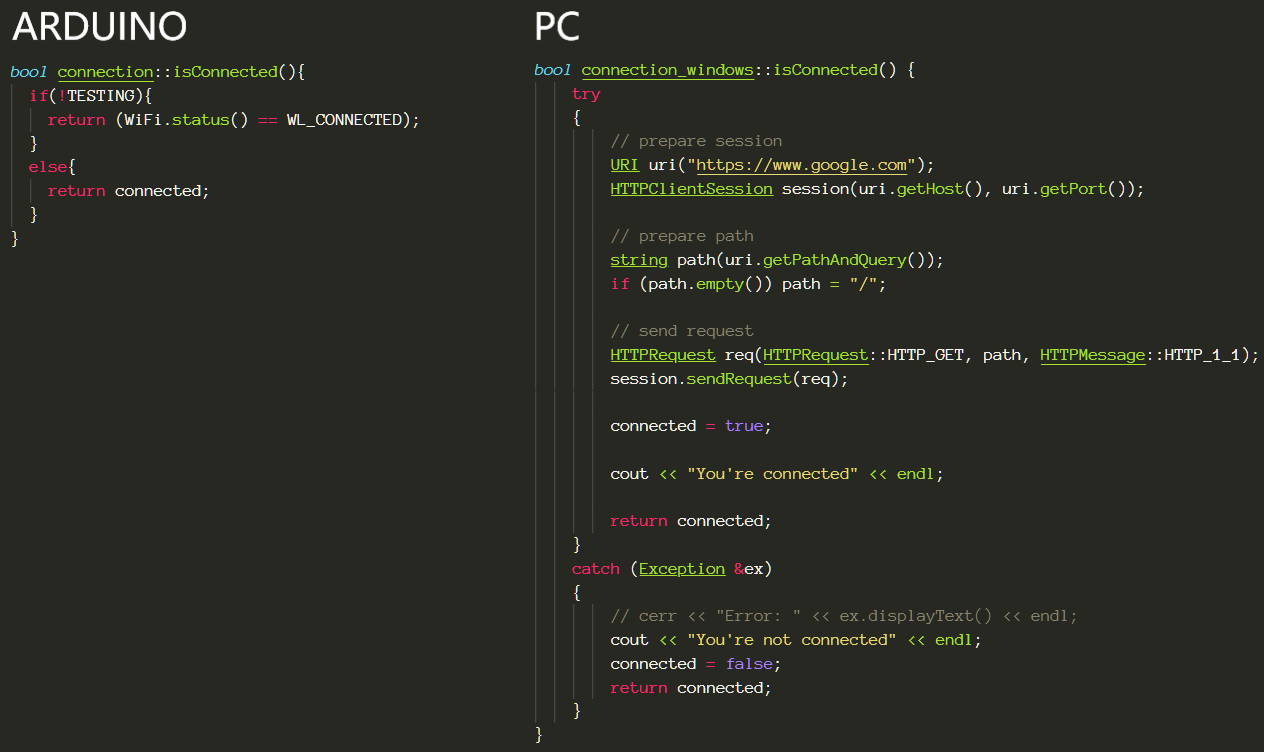
\includegraphics[width=\linewidth]{pics/connAW}
	\caption{Confronto tra le due implementazioni del metodo \texttt{isConnected}}
	\label{connAW}
\end{figure}

\subsection{APIRest\_windows}
La classe \texttt{APIRest} è un po' più complessa: fornisce un'interfaccia semplificata per l'uso di tutte le richieste HTTP(S) (nel progetto vengono usate solo GET e POST) celando i dettagli della libreria HTTPClient di Arduino. La sua istanza viene utilizzata sia dalla classe principale \texttt{edgine} sia dalla classe \texttt{postVal}, ultima operazione usata in ogni script che effettua la POST dei dati quando necessario. \texttt{APIRest} espone dunque i metodi necessari alla comunicazione con il Cloud occupandosi dei particolari implementativi della piattaforma utilizzata: preparazione dell'header e del body delle richieste, invio e gestione del responso. In seguito al fallimento di una richiesta di informazioni (GET), è l'engine a decidere come comportarsi e se comunicare l'errore al Cloud; se invece a fallire è la trasmissione di un dato o di un issue (POST) allora è questa stessa classe a memorizzare la richiesta fallita e a riprovarne l'invio fino alla corretta ricezione da parte del Cloud. Per ragioni principalmente energetiche questi tentativi vengono fatti ogni qualvolta si renda necessario effettuare l'invio di un nuovo dato e non in maniera continuativa. In ultimo, tale classe ha il compito di calcolare e fornire la data e l'ora correnti da allegare alle misurazioni e alle comunicazioni d'errore.

Dal momento che \texttt{APIRest} fa largo uso della libreria HTTPClient di Arduino, si è resa necessaria una nuova implementazione della stessa per dispositivi PC, \texttt{APIRest\_windows}. Questa classe ha il compito di svolgere le stesse funzioni dell’originale, ma, in questo caso, avvalendosi delle librerie POCO, al fine di rispettare le specifiche di compatibilità con altre piattaforme. In figura \ref{APIRestAW} è possibile notare le differenti implementazioni della funzione \texttt{POSTLogin}, adibita all'autenticazione sul Cloud e alla successiva ricezione del JWT.

\begin{figure}[H]
	\centering
	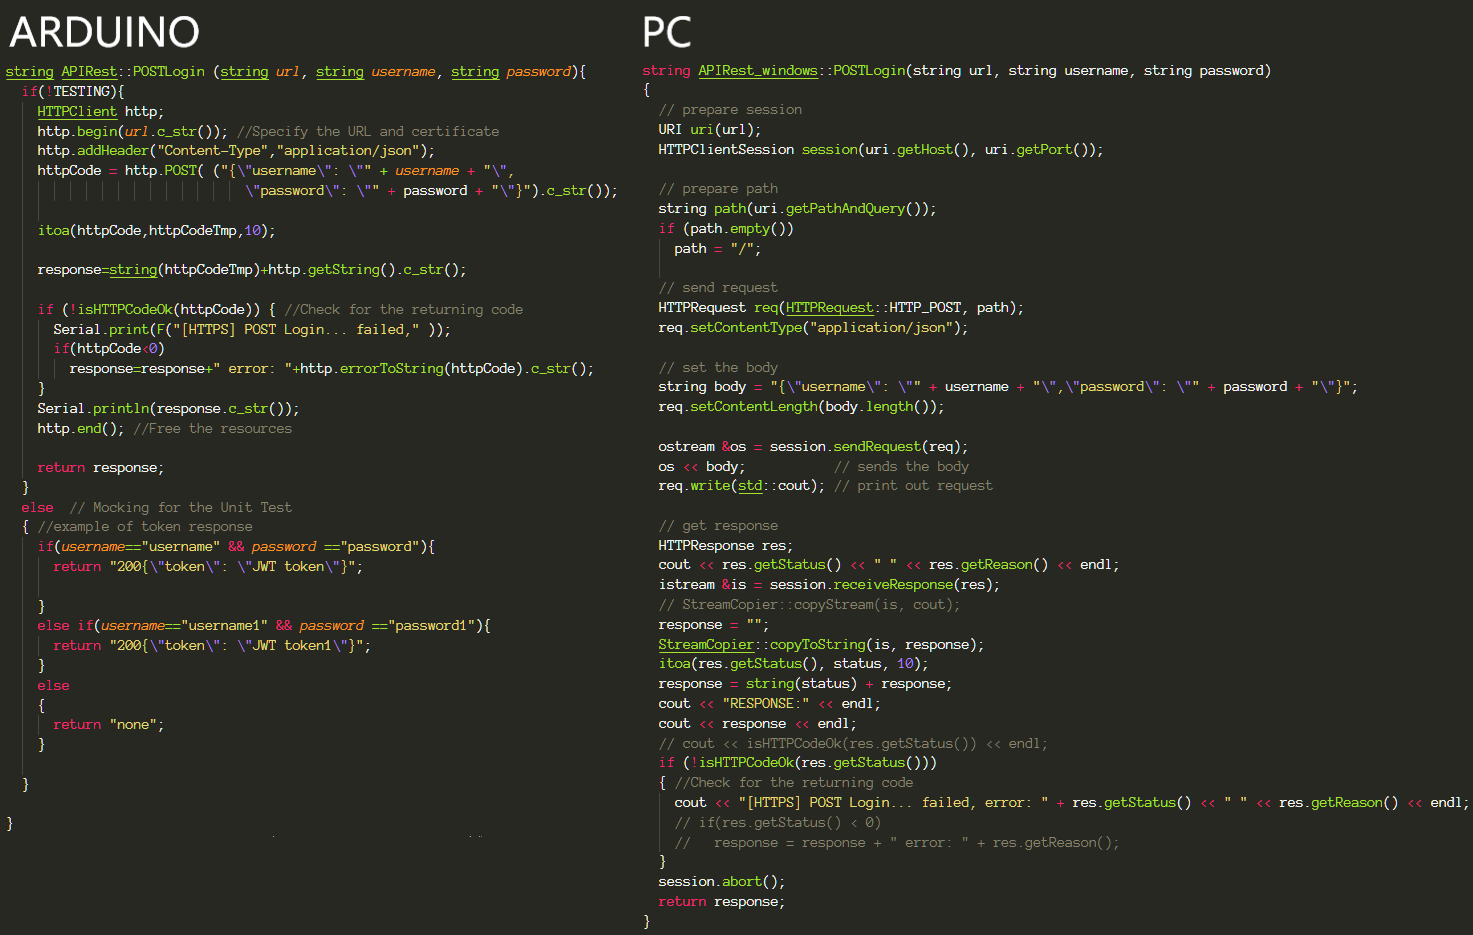
\includegraphics[width=\linewidth]{pics/APIRestAW}
	\caption{Confronto tra le due implementazioni del metodo \texttt{PostLogin}}
	\label{APIRestAW}
\end{figure}
\newpage

In primo luogo, il metodo prende in ingresso tre stringhe: url del server, username e password dell'utente necessari ad ottenere i permessi per accedere alle proprie risorse. In seguito viene eseguita una POST all'interno del cui body vengono specificati username e password, scritti in formato JSON. La response contiene lo stato della richiesta HTTP, che indica se l'operazione sia andata a buon fine o meno, e il JWT necessario per gli accessi futuri alle risorse.
\subsection{myDefines.h}

\begin{wrapfigure}{r}{6cm}
	\centering
	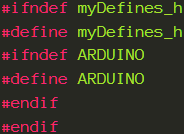
\includegraphics{pics/myDefines}
	\caption{myDefines.h}
	\label{myDefines}
\end{wrapfigure}

Una volta implementate le due classi wrapper \texttt{Connection\_windows} e \\\texttt{APIRest\_windows}, volendo mantenere la possibilità di passare da una piattaforma all'altra in modo rapido e semplice, si è scelto di creare un header file, \texttt{myDefines.h}, attraverso il quale fosse possibile decidere il target di esecuzione del proprio codice senza necessità di modificare ulteriori files. \texttt{myDefines.h} ha la struttura mostrata in figura \ref{myDefines}. Essa consiste semplicemente nella definizione della macro \texttt{ARDUINO} nel caso in cui si desideri compilare per tale piattaforma. Laddove invece tale macro non fosse definita, verrebbe scelta di default la compilazione per PC. \texttt{myDefines.h}, deve essere inclusa in tutti i file che utilizzano i metodi delle classi wrapper sopra descritte. All'interno di tali file, lo switch di piattaforma è gestito tramite direttive \texttt{\#ifdef}, come visibile in figura \ref{ifdef}.

\begin{figure}[H]
	\centering
	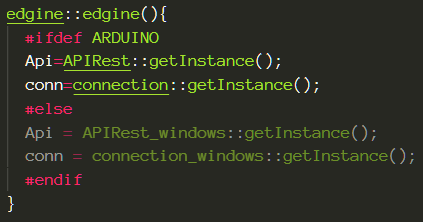
\includegraphics[width=0.66\linewidth]{pics/ifdef}
	\caption{Esempio di utilizzo della direttiva \texttt{\#ifdef}}
	\label{ifdef}
\end{figure}

In questa specifica situazione, nel caso in cui, come in figura, sia definita la macro \texttt{ARDUINO}, vengono create istanze delle classi \texttt{Connection} e \texttt{APIRest}, altrimenti delle classi \texttt{Connection\_windows} e \texttt{APIRest\_windows}.
\section{Esempio di prova}\label{prova}
Dopo aver ultimato l’implementazione delle classi citate in precedenza, si è deciso di sviluppare un semplice main per PC che simulasse un’applicazione IoT per il monitoraggio della temperatura, al fine di testare quanto realizzato.

Il device simulato possiede una feature: temperature. In prima istanza è necessario impostare tutti i parametri della descrizione virtuale e creare all'interno del Cloud la risorsa che rappresenti il dispositivo d’interesse. Dopodiché bisogna costruire gli scripts che si intende eseguire sui flussi di dati e assegnarli alla risorsa precedentemente creata sulle API di tale dispositivo. È necessario inoltre aggiungere un utente (parametri username e password nel codice) sul Cloud attraverso il quale l'engine potrà autenticarsi.

Il main è suddiviso in due fasi principali, associate alle funzioni \texttt{setup} e \texttt{loop} che richiamano la configurazione tipica degli sketch Arduino. Le procedure da svolgere nella funzione \texttt{setup} sono la configurazione del sensore, l'avvio della connessione Internet e l'assegnazione dei parametri alla struttura dati \texttt{options} per inizializzare l'engine. Nella funzione \texttt{loop} invece, è disposta la creazione dei sample (connotati da feature, data e valore letto dai sensori), poi processati dall'engine tramite gli script ricevuti dal Cloud. Tali script sono eseguiti ciclicamente e il risultato delle operazioni portate a termine viene conservato sul Cloud. Il processo di interazione Cloud-Edge appena descritto è riassunto nella tabella \ref{loop}. In questo specifico caso, siccome si tratta di un esempio di test e non di un'applicazione reale, la funzione \texttt{loop} viene eseguita una volta sola, dal momento che l'interesse non è l'invio dei dati in maniera iterativa, ma la verificare del funzionamento di un singolo script.

Già da un esempio semplice come quello appena descritto, ci si può rendere conto di come la realizzazione di un'applicazione IoT servendosi di Edge Engine riduca in maniera drastica la quantità di codice da produrre e il tempo di sviluppo del software. Esso fornisce la possibilità non solo di eseguire in locale gli script caricati da remoto, ma anche di inviare e ricevere delle informazioni dal Cloud e gestire eventuali malfunzionamenti, comunicandone l'avvenimento al server online.

\begin{table}[H]
	\centering
	\begin{tabular}{|l|l|l|}
		\hline
		\textbf{Request} & \textbf{Task} & \textbf{Descrizione}\\
		\hline
		\textbf{POST} & Credenziali di Login & Viene ricevuto il JWT dal Cloud\\
		\hline
		\textbf{GET} & Descrizione del device & Gli script vengono recuperati dal Cloud\\
		\hline
		\textbf{POST} & Measurements & I dati vengono salvati sul Cloud\\	
		\hline
	\end{tabular}
	\caption{HTTP requests generalmente eseguite da Edge Engine}
	\label{loop}
\end{table}

\section{Creazione della libreria}
Come è stato possibile notare nella sezione \ref{utilizzo}, il sistema, per poter essere utilizzato, necessita della compilazione di tutte le classi del progetto, andando dunque a rendere obbligatoria anche la presenza dei file \texttt{.cpp} (oltre agli header) all'interno del proprio ambiente di sviluppo. Questa procedura è assai utile in fase di implementazione del sistema, dal momento che in questo modo è possibile agire direttamente sulle classi in caso di errori o necessità di cambiamenti al codice. Tuttavia, non lo è altrettanto nel caso di utilizzo dell'Edge Engine da parte di sviluppatori che desiderino farne uso senza volontà di applicare modifiche al codice sorgente o qualora si desideri che la propria implementazione dei vari metodi non sia visibile a chi ne usufruisce.

Di conseguenza, si è deciso di creare un file \texttt{.lib} grazie al quale è facilitata la fruizione del sistema da parte di altri sviluppatori e, al contempo, viene nascosta la realizzazione relativa alle classi appartenenti al progetto.

Di seguito vengono mostrati i passaggi che è necessario eseguire per ottenere il file \texttt{.lib} a partire dal codice sorgente:

\begin{verbatim}
g++ -c APIRest_windows.cpp 
      -Ipath\to\EdgeEngine_library\src 
      -Ipath\to\msys64\mingw64\include 
g++ -c connection_windows.cpp 
      -Ipath\to\EdgeEngine_library\src 
      -Ipath\to\msys64\mingw64\include 

[...]

g++ -c window.cpp
      -Ipath\to\EdgeEngine_library\src 
      -Ipath\to\msys64\mingw64\include 
 
ar rcs Edgine.lib APIRest_windows.o connection_windows.o [...] 
      window.o
\end{verbatim}

I primi passaggi, da ripetere per ogni classe presente all'interno del progetto, producono per ognuna di esse il relativo file in formato \texttt{.o}, necessario per la successiva creazione del \texttt{.lib}. Il comando \texttt{ar} poi, a partire da i file \texttt{.o} appena creati, genera la libreria \texttt{Edgine.lib}. Infine, per poterla utilizzare all'interno del proprio progetto, sono necessarie le seguenti direttive per il compilatore:

\begin{verbatim}
-g
main.cpp
-o
main.exe
-Ipath\to\library\repository\include
-Ipath\to\msys64\mingw64\include
-Lpath\to\library\repository\lib
-Lpath\to\msys64\mingw64\lib
-lEdgine
-lPocoFoundation
-lPocoUtil
-lPocoNet
\end{verbatim}








